\documentclass[11pt]{article}

\usepackage{fullpage}
\usepackage{color}
\newcommand{\BKM}[1]{\textcolor{blue}{BKM: #1}}
\newcommand{\RNG}[1]{\textcolor{red}{RNG: #1}}

\usepackage[export]{adjustbox}
\usepackage{fancyhdr}
\pagestyle{fancy}
\fancyhf{}
\rfoot{\thepage}
\cfoot{
\includegraphics[height=0.6in,valign=c]{LetterheadFooter}}
\renewcommand{\headrulewidth}{0pt}

\newenvironment{response}
{\begin{quote}\itshape}
{\end{quote}}

\setlength{\parindent}{0em}
\setlength{\parskip}{0.5em}

\usepackage{xr}
\externaldocument{NAR_DRAFT}

\begin{document}
\vspace*{-0.5in}\hspace*{-0.2in}
\includegraphics{LetterheadHeader}\vspace*{\baselineskip}

\noindent Dear Professor Herrero,

We appreciate the opportunity to revise our manuscript for publication in \emph{NAR Genomics and Bioinformatics}, and we thank you and the reviewers for the quality of the reviews. Below we respond in italics to the reviewers' concerns.

\noindent Sincerely,\\
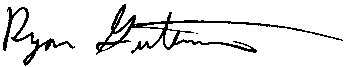
\includegraphics{signature}\\
Ryan Gutenkunst, PhD\\
Associate Professor and Associate Department Head\\
Department of Molecular and Cellular Biology\\
University of Arizona

\section*{Associate Editor}

Stressing on some of the points raised by the reviewers, I would suggest you include more details about the assumption and limitations of BATCAVE. In particular, the possibility of changes of mutational signatures over time can be quite striking in some cases, especially if the original tumour is driven by very specific mutagens like UV light or tobacco smoke. Ideally, the software should try to correct for these cases or at least warn the user about a possible shift in signatures/contexts.
\begin{response}
As we noted in the Discussion, BATCAVE does assume that the mutation profile is similar between mutations that are high-confidence (tend to be earlier) and low-confidence (tend to be later).
Modeling potential changes in the profile is beyond the scope of the current manuscript, but warning the user if such a shift exists is a great idea.
We have thus implemented a statistical test as to whether the mutation profile from the high-confidence mutations differs significantly from the low-confidence mutations.
If this test detects a difference, BATCAVE warns the user and outputs both profiles, so the user can assess the degree of difference and follow-up on any potential biological implications.

When we reanalyzed our test data using this new approach, we did detect a profile shift in the AML data.
Note that even with this shift, BATCAVE still performs better than MuTect on the validated mutations (although both perform extremely well).
\RNG{The biology of the shift is...}
\end{response}

Related to this, there is probably a minimum number of high-confidence mutations that are required by BATCAVE to produce reliable results. As with the previous point, ideally the batcaver should address or warn the user if the assumptions are violated.
\begin{response}
Our simulation studies suggest that a few hundred high-confidence mutations are enough to reliably infer even a sharply peaked mutation profile (Fig. 3).
We have modified \texttt{batcaver} so that it now emits a warning if there are fewer than 500 high-confidence mutations in a sample.
\end{response}

Lastly, as correctly pointed out by the second reviewer, the sequencing coverage only makes sense in the context of the purity of the samples and this information should be provided to the reader.
\begin{response}
The direct effect of contamination by normal cells on the BATCAVE algorithm is to bias the estimated allele frequencies that are inputs to Eq.~11 for estimating the overall mutation rate.
This bias can be simply corrected given an estimate of tumor purity.
We have thus added a \texttt{--tumor\_purity} option to \texttt{batcaver}.
When this is enabled, the estimated allele frequencies will be appropriately adjusted before applying Eq.~11.
See new text in Methods for details.

We also reanalyzed our real data examples, using purity estimates from the original publications.
\RNG{
The effect of accounting for tumor purity was to...
We have updated the text, Table~1, and Fig.~4E\&F to reflect these new results.
}
 
\end{response}


\section*{Reviewer 1}

Mannakee and Gutenkunst present BATCAVE, an algorithm that first estimates the tumor’s mutation profile and mutation rate using high-confidence variants and then uses them as a prior when calling other variants based on mutational signatures. The concept behind this work is interesting. However, the difference in accuracy between MuTect and BATCAVE is relatively small except for the case when one has particularly high depth sequencing (500x), limiting the utility of the method. 

Still, the 500x whole exome case does indicate that BATCAVE is better at identifying low frequency variants and thus can better reveal intratumoral heterogeneity, an important area of inquiry in cancer. Interestingly, the AUROC values for both MuTect and BATCAVE have room for improvement for the 500x whole exome case (Table 1). I suggest the authors further investigate how to improve the AUROC values. For example, in equation 4, it is unclear why the authors assume $\nu$ be uniformly distributed. Although this is also an assumption of MuTect, the BATCAVE approach inherently distinguishes mutations by allele frequency – since log-likelihood is closely associated to AF.  Perhaps a model in which $\nu$ follows a decreasing distribution vs. AF (e.g. in concordance with a model of a growing tumor) would yield better AUROC values.  
\begin{response}
A uniform prior over $\nu$ is appropriate when the goal is to make the best possible call at each potential variant site.
Conceptually, before examining the read data we have no information about the allele frequency at any individual site.
Practically, a nonuniform prior would favor low-frequency and thus typically low-evidence sites, increasing the false positive rate.
If our goal were to best estimate the distribution of variant allele frequencies in the tumor, then a nonuniform $\nu$ would indeed be important.

We discuss this issue in a new paragraph in Discussion.
\end{response}

In Rubanova et al ( https://www.biorxiv.org/content/10.1101/260471v4.full), it is argued that there are changes in mutational signatures over time in cancers. While Mannakee and Gutenkunst mention this work, they should further comment on whether such changes in mutational signatures over time are small enough to be explained by the BATCAVER concept of re-evaluating mutations based on p-value.
\begin{response}
We cannot comment generally on the magnitude of mutation profile changes, because this is an developing area of research.
But to protect users, we have implemented a new statistical test to detect changes in mutation profiles between high- and low-confidence mutations.
See our response to the Associate Editor for more details.
\end{response}

Minor
p.2: “Folding the central base to the pyrimidines”: The “folding” terminology is not standard and should be improved. 
\begin{response}
Corrected
\end{response}

Equation 11: This equation is not correct if there is subclonal copy number evolution that changes the distribution of mutations above the allele frequency threshold. The authors should more clearly state this assumption.
\begin{response}
The reviewer is correct, although a large number of copy number changes would be necessary to substantially bias the estimated mutation rate.
Potential future work could incorporate external copy number calls to improve the estimate of the point mutation rate.

We discuss this issue in a new paragraph in Discussion.
\end{response}

\section*{Reviewer 2}

Mannakee et al have developed a tool called BATCAVE for calling mutations from sequencing data. They claim to have used a novel approach of using tumor and site-specific priors for calling mutations. In my opinion authors have done a good job in terms of using a novel approach which harnesses patient/tumor specific information to call mutations. I agree with the authors that this approach was missing in other tools. I accept this study to be published given the authors address few points mentioned below:

1. Does BATCAVE accounts for tumor purity estimates while calling mutations?
\begin{response}
We neglected to account for the effect of tumor purity on mutation rate estimation from Eq.~11.
We have corrected this omission.
Please see our response to the Associate Editor's comment for details.
\end{response}

2. In case of multi-region sequencing data, used for studying spatial intra-tumor heterogeneity, usually the existing tools estimate very high levels of heterogeneity. I suppose this is because they are being very stringent in terms of calling mutations especially the ones with low vafs. In that case the people end up using other tools like bamreadcount etc. to check status of these mutations in the bam files and re-estimate the extent of heterogeneity. It will be important to see how BATCAVE performs in such datasets.
\begin{response}
We agree that multi-region data are increasingly important.
In fact, the breast cancer data we test on come from a multi-region study. 
Because we built BATCAVE on top of the single-sample caller MuTect, we called variants independently across the samples in that study, and BATCAVE performed well.
Unfortunately, the sequencing in that study is not deep enough to rigorously evaluate how estimates of heterogeneity would change with and without BATCAVE.

More broadly, the BATCAVE algorithm could be implemented in a multi-regional caller that takes explicit advantage of the relationship between samples.
But such an implementation is beyond the scope of the current manuscript.

We have added a new paragraph in Discussion regarding multi-region samples, to address these issues.
\end{response}

3. Do the mutation signatures (example smoking signatures in lung cancer or UV signatures in melanoma) still appear in the more stringent BATCAVE set of mutations?
\begin{response}
In our real and simulated test cases, the mutational profile changes little between high- and low-confidence sets of mutations.
In fact, we have added a statistical test for profile change, in response to other review comments.

Approaches such as deconstructSigs can decompose an individual sample's mutational profile into a set of mutation signatures corresponding to different processes.
In practice, however, we have found these approaches to be relatively unstable.
Therefore, we do not believe it will be illuminating to apply them in the present manuscript.
\end{response}

\end{document}
